%!TEX root = ./main.tex
%!TEX encoding = UTF-8 Unicode
\chapter{Description de la syntaxe des instructions}
\label{chap:syntax}
\section{Introduction}
Dans ce chapitre, nous allons présenter comment décrire la syntaxe du jeu d'instructions d'un processeur donné, en se servant de quelques exemples extrait de la description de HCS12 de Freescale et de son co-processeur XGate, ainsi que de la description de l'AVR.

La vue syntaxique suit le même principe que les deux autres. Elle décrit le format textuel des instructions, en concaténant des chaînes de caractères. En d'autres termes, elle permet d'attribuer une syntaxe textuelle pour chaque signature d'instruction pour permettre, par exemple, le désassemblage. 

\section {Structure arborescente de la vue syntaxique dans \harmless}
Comme dans les deux autres vues (binaire et sémantique), la vue syntaxique est composée d'un ensemble d'arbres, dans lesquels un nœud décrit une partie de la syntaxe d'une ou plusieurs instructions. Chaque branche de l'arbre représente une instruction.

Dans cette vue, chaque nœud suit la syntax suivante:

\begin{lstlisting}
syntax <name> [etiquette]
  <syntaxBody>
end syntax
\end{lstlisting}

Un nœud \texttt{syntax} peut "appeler" un autre nœud, ou faire une structure de sélection entre différents nœuds, à l'aide d'une structure de type \texttt{select}. Cette approche est commune aux 4 vues (\texttt{format}, \texttt{syntax}, \texttt{behavior} et \texttt{timing}) et est décrite plus en détails à la section \ref{sec:modelisationArborescente}.

Nous allons ici nous intéresser plus particulièrement au corps d'un nœud \texttt{<syntaxBody>} qui est spécifique à la génération d'un mnémonique, tout en donnant quelques exemples liés à la structure arborescente de la description des éléments de type \texttt{syntax}.

\section{La partie \texttt{<syntaxBody>}}

La partie \texttt{<syntaxBody>} est une succession d'éléments de type (\ref{sec:syntaxBody}):
\begin{itemize}
\item \emph{étiquette};
\item étiquette (l'ensemble des étiquettes définissant la signature de l'instruction), voir \ref{sec:syntaxEtiquette};
\item appel à un autre nœud de type \texttt{syntax}, en utilisant le nom de l'élément \texttt{syntax} appelé;
\item structure de sélection, en utilisant le mot clé \texttt{select}, voir section \ref{sec:syntaxSelect};
\item déclaration de \emph{field}, voir section \ref{sec:syntaxField};
\item chaîne de caractères suivie ou non d'un ou plusieurs variables déclarées. Cette chaîne constitue le mnémonique à proprement parler de l'instruction, voir section \ref{sec:syntaxChaineCaract};
\item structure de sélection permettant de mettre en œuvre un choix dynamiquement (en fonction de la valuer des données), voir section \ref{sec:syntaxIf}.
\end{itemize}

\subsection{Les étiquettes}
\label{sec:syntaxEtiquette}
Comme dans la vue binaire, les nœuds sont associés à des étiquettes (tags) dont l'ensemble forme la signature de l'instruction. Lors de l'évaluation des différents chemins des instructions, les étiquettes sont récoltées pour former la signature de l'instruction. On s'intéresse à un \emph{ensemble}, donc le nombre d'étiquettes de même nom n'est compté qu'une fois, et il n'y a pas de relation d'ordre, voir \ref{sec:signature}.

\subsection{Structure de sélection \texttt{select}}
\label{sec:syntaxSelect}
Le mot clé {\tt "select"} permet de créer différentes branches dans l'arborescence, comme indiqué dans \ref{sec:modelisationArborescente}.

La syntaxe générale de cette structure est la suivante:
\begin{lstlisting}
syntax test
  <syntaxBody1>
  select 
    case <syntaxBody2>
    case <syntaxBody3>
    ...
  end select;
  <syntaxBody4>
end syntax
\end{lstlisting}
Ainsi, dans cette architecture, 2 instructions sont définies. Elles sont composées respectivement des éléments:
\begin{itemize}
\item \texttt{<syntaxBody1>}, \texttt{<syntaxBody2>} et \texttt{<syntaxBody4>};
\item \texttt{<syntaxBody1>}, \texttt{<syntaxBody3>} et \texttt{<syntaxBody4>};
\end{itemize}
 Ainsi, la structure \texttt{select} permet de mutualiser les parties communes aux mnémoniques de différentes instructions (\texttt{<syntaxBody1>} et \texttt{<syntaxBody4>}), et de les différencier sur d'autres parties.

Bien entendu, les étiquettes dans les parties \texttt{<syntaxBody2>} et  \texttt{<syntaxBody3>} doivent être différentes pour différencier les différents chemins (et constituer les signatures des instructions).

Soit par exemple (issu du jeu d'instructions de l'AVR):
\begin{lstlisting}
syntax classicImm8 
  field u4 regIndex -- should add 16 to the result
  field u8 k
  select
    case #ANDI "ANDI" -- or CBR with ~k 
    case #CPI  "CPI"
    case #ORI  "ORI"
    case #SBCI "SBCI"
    case #SUBI "SUBI"
  end select
  " R\d, \x", regIndex+16, k
end syntax
\end{lstlisting}
Cet exemple permet de construire la syntaxe de 5 instructions différentes, en mutualisant la récupération des champs issus du \texttt{format}, ainsi que leur affichage. Dans ce cas, les signatures des instructions ne comprennent qu'une seule étiquette.

Cette structure en \texttt{select} est résolue de manière statique à la génération du simulateur. Par conséquent, 5 instructions seront générées, avec chacune leur code associé. Aucun impact sur les performances n'est associé à la multiplication des éléments \texttt{select}.

\subsection{Récupération des champs du format binaire}
 \label{sec:syntaxField}
 Dans la vue syntaxique, il est nécessaire de pouvoir récupérer la valeur des différents champs extrait du code binaire de l'instruction. L'opération d'extraction de ces champs dans la partie binaire de l'instruction est réalisé dans la partie \texttt{format} de la description. Dans la partie \texttt{syntax}, on se contente de récupérer ces différents champs sous la forme de constantes.
 
 Ainsi, le mot clé {\tt "field"} permet de référencer un champ qui est extrait de l'instruction dans la vue binaire.\harmless\ étant un langage fortement typé, le type des différents champs doit correspondre exactement avec celui extrait de la vue binaire:

\begin{lstlisting}
field <typeDonnee> <nom_du_champ>
\end{lstlisting}

Où {\tt <typeDonnee>} est un type de donnée, comme défini dans la section \ref{sec:TypeDonnees} (\texttt{u3} pour un entier non signé sur 3 bits, \texttt{s5} pour un entier signé sur 5 bits, \ldots). Il doit correspondre au nombre de bits extraits dans la vue binaire pour la même variable (ou être plus grande).

Par exemple, une donnée non signée nommée {\tt "rs1Index"} est déclarée dans la vue binaire de la façon suivante:

\begin{lstlisting}
rs1Index := slice{7..5}
\end{lstlisting}

Dans la vue syntaxique, sa valeur sera importée sous la forme:

\begin{lstlisting}
field u3 rs1Index
\end{lstlisting}

Ici, nous pouvons remarquer que la taille du champ est égale à 3, ce qui correspond bien au 3 bits extraits (bit 7, 6 et 5).

\subsection{Les  chaînes de caractères}
\label{sec:syntaxChaineCaract}
Dans la vue syntaxique, une chaîne de caractères est une suite de caractères entre guillemets. 

Lors de l'évaluation d'une branche de la description (qui modélise une instruction), les différentes chaînes de caractères sont concaténées pour former la mnémonique de l'instruction.

Avec une approche similaire à celle de la fonction \texttt{printf} du langage \texttt{C}, il est possible de faire référence à des données qui sont définies en dehors de la chaîne de caractères, en utilisant des séquences d'échappement. Chaque séquence d'échappement est alors remplacée par une expression:

\begin{lstlisting}
<chaine_de_caracteres>, <expression_0>, ..., <expression_n>
\end{lstlisting}

soir par exemple:
\begin{lstlisting}
    "CLR R\d", rdIndex
    ...
    "LDI R\d, \x", regIndex+16, k
\end{lstlisting}
Il est indispensable d'avoir le même nombre de caractères d'échappements que d'expressions.

\subsubsection{Séquences d'échappement dans les chaînes de caractères}
Les séquences d'échappement permettent de faire référence aux expressions qui suivent la chaîne de caractère. Les 4 séquences d'échappement permettent de définir la base utilisée pour l'affichage:
\begin{table}[!h]
\begin{center}
\begin{tabularx}{0.7 \columnwidth}{|X|c|}
\hline
\bf séquence d'échappement & \bf Signification \\  \hline
\textbackslash b & Base binaire \\ \hline
\textbackslash d & Base décimal \\ \hline
\textbackslash x & Base hexadécimal \\ \hline
\textbackslash o & Base octal \\ \hline
\end{tabularx}
\caption{Base utilisée pour les différentes séquences d'échappement}
\label{tab:type-donnee}
\end{center}
\end{table}

De plus, pour chaque base, \harmless\ donne la possibilité de préciser les caractères avant (\texttt{prefix}) et après (\texttt{suffix}) l'expression de manière globale, selon la syntaxe suivante: 

\begin{lstlisting}
number syntax <base> <prefix_ou_suffix> <chaine_de_caracteres>
\end{lstlisting}

Où {\tt <base>} peut être {\tt binary, octal, hexadecimal} ou {\tt decimal}. {\tt <prefix\_ou\_suffix>} peut être {\tt prefix} ou {\tt suffix}, et \texttt{<chaine\_de\_caracteres>} est une suite quelconque de caractères entres guillemets. Ces directives sont généralement placées au début de la section où sont placés les éléments \texttt{syntax}.
Voici un exemple: 

\begin{lstlisting}
number syntax octal prefix "o"
number syntax hexadecimal prefix "0x"
number syntax hexadecimal suffix "h"
\end{lstlisting}

Ainsi, à travers cet exemple, la description suivante:
\begin{lstlisting}
    "LDI R\d, \x", regIndex+16, k
\end{lstlisting}
conduira à l'affichage suivant (si k=5, et regIndex = 3):
\begin{verbatim}
    "LDI R19, 0x5h"
\end{verbatim}

\subsection{La structure \texttt{if ... then ... else}}
\label{sec:syntaxIf}
La structure conditionnelle \texttt{if ... then ... else} permet de faire un choix dynamique en fonction des différents champs d'une instruction. Elle est utilisée de la manière suivante:
\begin{lstlisting}
if <condition> then
  <ifSyntaxStatement>
[elseif <condition> then
  <ifSyntaxStatement>
]
[else 
  <ifSyntaxStatement>
]
end if;
\end{lstlisting}

La \texttt{<condition>} est une expression booléenne classique (voir \ref{sec:expressions}).
La partie \texttt{<ifSyntaxStatement>} n'est prise en compte que si la condition est vraie. On peut avoir:
\begin{itemize}
\item une chaîne de caractères;
\item une autre condition (\texttt{if..then..end if}.
\end{itemize}

Par contre, comme la condition est évaluée dynamiquement (à l'exécution), il n'est pas possible de faire intervenir des informations qui sont utilisées statiquement (au moment de la génération des sources du simulateur), comme par exemple une étiquette ou une structure de type \texttt{select}.

Les parties {\tt "elseif"} et {\tt "else"} sont facultatives.

Cette approche permet notamment de définir les \emph{mnémoniques simplifiées} associées à certaines instructions. Dans l'exemple suivant, une instruction de type \texttt{OR Rd, Ra, Ra} est simplifiée en \texttt{MOV Rd, Ra}:
\begin{lstlisting}
syntax orOperation #TriadicInst #OR
  field u3 rs1Index
  field u3 rs2Index
  field u3 rdIndex
  if rs1Index = rs2Index then
    "MOV R\d, R\d", rdIndex, rs1Index
  else
    "OR R\d, R\d, R\d", rdIndex, rs1Index, rs2Index
  end if;
end syntax
\end{lstlisting}

\section{Assemblage du tout}

Prenons comme exemple l'ensemble d'instructions faisant intervenir 3 registres dans la XGate. Dans la documentation technique, cet ensemble d'instructions est résumé par le tableau \ref{tab:triadic}.

\begin{table}[!h]
\begin{center}
\begin{tabularx}{1.1 \columnwidth}{|c|c|c|c|c|c|c|c|c|c|c|c|c|c|c|c|X|} 
\hline
\bf Functionality & \bf 15 & \bf 14 & \bf 13 & \bf 12 & \bf 11 & \bf 10 & \bf 9 & \bf 8 & \bf 7 & \bf 6 & \bf 5 & \bf 4 & \bf 3 & \bf 2 & \bf 1 & \bf 0\\  \hline
\bf Logical triadic & \multicolumn{16}{c|}{ } \\ \hline
AND RD, RS1, RS2 & 0 & 0 & 0 & 1 & 0 & \multicolumn{3}{c|}{RD} & \multicolumn{3}{c|}{RS1} & \multicolumn{3}{c|}{RS2} & 0 & 0 \\ \hline
OR RD, RS1, RS2 & 0 & 0 & 0 & 1 & 0 & \multicolumn{3}{c|}{RD} &  \multicolumn{3}{c|}{RS1} & \multicolumn{3}{c|}{RS2} & 1 & 0 \\ \hline
XNOR RD, RS1, RS2 & 0 & 0 & 0 & 1 & 0 & \multicolumn{3}{c|}{RD} & \multicolumn{3}{c|}{RS1} & \multicolumn{3}{c|}{RS2} & 1 & 1 \\ \hline
\bf Arithmetic triadic & \multicolumn{16}{c|}{For compare use SUB R0,Rs1,Rs2} \\ \hline
SUB RD, RS1, RS2 & 0 & 0 & 0 & 1 & 1 & \multicolumn{3}{c|}{RD} & \multicolumn{3}{c|}{RS1} & \multicolumn{3}{c|}{RS2} & 0 & 0 \\ \hline
SBC RD, RS1, RS2 & 0 & 0 & 0 & 1 & 1 & \multicolumn{3}{c|}{RD} & \multicolumn{3}{c|}{RS1} & \multicolumn{3}{c|}{RS2} & 0 & 1 \\ \hline
ADD RD, RS1, RS2 & 0 & 0 & 0 & 1 & 1 & \multicolumn{3}{c|}{RD} & \multicolumn{3}{c|}{RS1} & \multicolumn{3}{c|}{RS2} & 1 & 0 \\ \hline
ADC RD, RS1, RS2 & 0 & 0 & 0 & 1 & 1 & \multicolumn{3}{c|}{RD} & \multicolumn{3}{c|}{RS1} & \multicolumn{3}{c|}{RS2} & 1 & 1 \\ \hline
\end{tabularx}
\caption{Ce tableau représente l'ensemble d'instructions  {\tt "triadic"}, comme trouvé dans le datasheet de la XGate.}
\label{tab:triadic}
\end{center}
\end{table}

Dans  \harmless\ , cet ensemble d'instructions peut être décrit comme suit:
 
\begin{lstlisting}
syntax triadicInstruction #TriadicInst 
  field u3 rs1Index
  field u3 rs2Index
  field u3 rdIndex
  triadicOperation
  " R\d, R\d, R\d", rdIndex, rs1Index, rs2Index
end syntax

syntax triadicOperation 
  select
    case #AND  "AND"
    case #XNOR "XNOR"
    case #SBC  "SBC"
    case #ADD  "ADD"
    case #ADC  "ADC"
  end select
end syntax

syntax orOperation #TriadicInst #OR
  field u3 rs1Index
  field u3 rs2Index
  field u3 rdIndex
  if rs1Index = rs2Index then
    "MOV R\d, R\d", rdIndex, rs1Index
  else
    "OR R\d, R\d, R\d", rdIndex, rs1Index, rs2Index
  end if;
end syntax

syntax subOperation #TriadicInst #SUB
  field u3 rs1Index
  field u3 rs2Index
  field u3 rdIndex
  if rdIndex = 0 then
    "CMP R\d, R\d",rs1Index, rs2Index
  else
    "SUB R\d, R\d, R\d", rdIndex, rs1Index, rs2Index
  end if;
end syntax

\end{lstlisting}

La vue syntaxique a une structure arborescente, dont la représentation graphique est donnée dans le schéma \ref{fig:TriadicInst}. On peut noter que les 2 premiers éléments \texttt{syntax} permettent de traiter les cas généraux, et que les 2 suivants permettent de traiter des cas particuliers (car contenant des mnémoniques simplifiées).

\begin{figure}		
  \begin{center}
    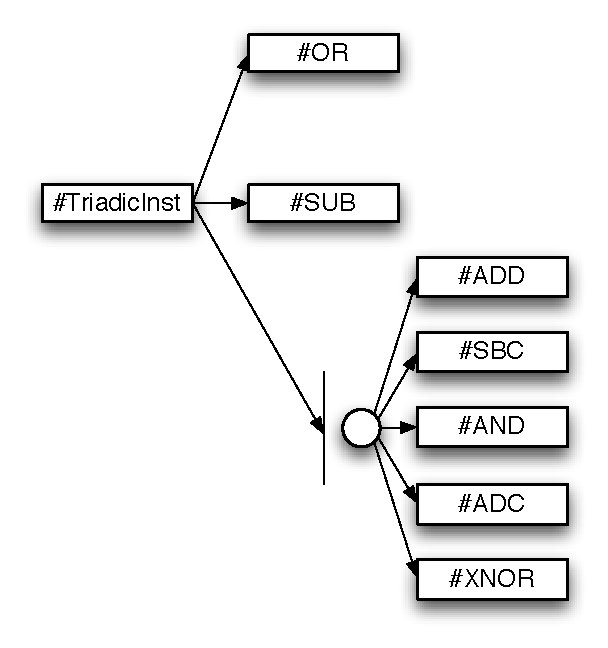
\includegraphics[width=0.5 \linewidth]{../common/images/TriadicInst.pdf}
    \caption{Syntaxe de l'ensemble d'instructions triadic.}
    \label{fig:TriadicInst}
  \end{center}
\end{figure}
